% ENEL 617 Radio Frequency Integrated Circuits Project Report
% Pouyan Keshavarzian
% Winter 2017
% Master's of Science in Electrical Engineering studies

%-------------------------------------------------------------------------------
% DOC SETUP
\documentclass{article}                                                         % document type
\usepackage[margin=0.7in]{geometry}                                             % Set margins
\usepackage{hyperref}                                                           % Enables typesetting of hyperlinks
\usepackage{float}                                                              % Required to keep images where they are put
\usepackage[dvipsnames]{xcolor}                                                 % More colors!
\usepackage{graphicx}                                                           % Required for the inclusion of images
\usepackage{listings}                                                           % Required for the inclusion of source code
\usepackage{mathtools}                                                          % Math looks pretty. Main backbone is amsmath
\usepackage{enumitem}                                                           % Required to use different characters for enumerated lists
\usepackage{multirow}                                                           % Create tabular cells spanning multiple rows
\usepackage[toc]{glossaries}                                                    % Create glossary
\usepackage[titletoc]{appendix}                                                 % Create Appendix
\usepackage{wrapfig}                                                            % Needed for wrapping text around a figure
\usepackage{subfig}                                                          % Subfigures
%\usepackage[]{mcode}                                                           % Matlab code
\setlength\parindent{0pt}                                                       % Removes all indentation from paragraphs
\providecommand{\e}[1]{\ensuremath{\times 10^{#1}}}                             % Use scientific notation
%\usepackage{times}                                                             % Uncomment to use the Times New Roman font
\usepackage{pdfpages}                                                           % Simplifies inclusion of external multi-page pdfs into document
\loadglsentries[main]{glossary}                                                 % Glossary
\makeglossaries
\usepackage[backend=bibtex, firstinits=false, style=ieee]{biblatex}
\addbibresource{Bibliog.bib}
\usepackage{verbatim}                                                           % Does things verbatim?? For example \verbatiminput{appendices/GuitarTunerApp.mc}. Also adds \begin{comment}. Also reporduces text verbatum
\usepackage{pdflscape}                                                          % For landscape pages

%-------------------------------------------------------------------------------
%----------------------------------------------------------------------------------------
%	DOCUMENT TITLE PAGE
%----------------------------------------------------------------------------------------
\title{\textsc{\textbf{ENEL 617 WINTER 2017 PROJECT REPORT}}} % Title
\author{\textsc{Millimeter-Wave Double Balanced Gilbert Mixer}
\\ \textsc{Pouyan Keshavarzian}}
\date{\today} % Date for the reports
\begin{document}
\maketitle % Insert the title, author and date
\newpage
%----------------------------------------------------------------------------------------
%	Table of Contents and Figures
%----------------------------------------------------------------------------------------
% Add tables and lists as required
\tableofcontents
\listoffigures
\listoftables
%-------------------------------------------------------------------------------
\newpage
%----------------------------------------------------------------------------------------
%	GLOSSARY
%----------------------------------------------------------------------------------------
\section{Glossary}
\printglossary[title=Terms Acronyms and Abbreviations]
\newpage
%----------------------------------------------------------------------------------------
%	SECTION
%----------------------------------------------------------------------------------------
\section{PROJECT MOTIVATION}
In this project, I present a double balanced mixer that would be used as part of a  BPSK Modulator circuit
to generate a spread spectrum radar waveform in the automotive frequency band (77-81 GHz). A similar modulator
that uses a double-balanced mixer is described in [CITE]. The original design benchmarks for this mixer
and the achieved final results are outlined in Table ~\ref{table:goalsnresults}.\vspace{3mm}
\vspace{3mm}
\begin{table}[H]
\centering
 \begin{tabular}{ | c | c | c |}
   \hline
    \textbf{Parameter} & \textbf{Original} & \textbf{Achieved}  \\
    \hline
    \hline
    Supply Voltage & 1.8V & 0.85V \\
    \hline
    Power Consumption & 5mW & $\approx$ \textbf{\textcolor{OliveGreen}{4.8mW}}\\
    \hline
    Gain (dB)   & 5 & $\approx$ \textbf{\textcolor{Red}{-13 dB}} \\
    \hline
    Input Match  & 50$\Omega$ & \textbf{\textcolor{OliveGreen}{45.5 + j0.1$\Omega$}} \\
    \hline
    Output Match & 730$\Omega$ & \textbf{\textcolor{Orange}{48.9 + j0.1$\Omega$}}\\
    \hline
    NF & 10dB & $\approx$ \textbf{\textcolor{Red}{16 dB}}\\
    \hline
    P1dB & -- & $\approx$ 1.5dB  \\
    \hline
    IP3 & -- & $\approx$ 9.5dB  \\
    \hline
  \end{tabular}
  \caption{Mixer Design Goals}
  \label{table:goalsnresults}
\end{table}
The original values were generated based on a few simple simulations/calculations and a power budget provided by Dr. Belostotski. The
power budget was the control variable that I set as an absolute requirement.  Once the Id-gm
characteristics were understood from simulation, the gain estimate was calculated using the following equation.
\begin{equation}
  \label{eq:idealgain}
  G=\dfrac{2}{\pi}\dfrac{R_L}{R_s + \dfrac{1}{g_m}};
\end{equation}
The exact values including plots for the final results will be clearly outlined. Furthermore, deviations from original to achieved results
will be described in detail. A different design topology was used in the final design than in the original biased circuit used to calculate
the conversion gain. Some targets (such as output impedance) were changed intentionally (for practical purposes) while other values
were adjusted based on non-ideal aspects of the circuit.\vspace{3mm}
A derivation of Equation ~\ref{eq:idealgain} will be provided in the theory of operation section. A suitable value of $R_L$ was chosen
based on biasing and achieving high gain. This value, and others, deviate greatly from the final design. A thorough explanation of the
reasons for deviating are provided.
The interest in this particular-type of radar stems from spread-spectrum technology's built in interference rejection, which
is an indispensable feature for automotive radar. This type of radar has recently been demonstrated in
SiGe technology [CITE]. 65nm technology is chosen because the Figure of Merit, $f_T \approx 160GHz $, making it suitable for
this millimeter-wave application.

\subsection{Radar Theory of Operation}

\begin{wrapfigure}{r}{0.5\textwidth}
  \begin{center}
    \includegraphics[width=0.4\textwidth] {Figures/radarblock.png}
    \caption{Radar Transceiver Block Diagram}
    \label{fig:radartrans}
  \end{center}
\end{wrapfigure}
To demonstrate how this mixer could be used in a practical application, the theory of the type of radar is discussed.
A simplified block diagram of an example spread spectrum ranging system is shown in Figure ~\ref{fig:radartrans}.
The BPSK modulator is used to spread the carrier with a pseudorandom code. The parameters of the code, which govern
the LO mixing frequency, are designed to provide an adequate range resolution within the context of automotive radar.
The achievable range resolution of the radar system is related to the chip rate (mixer LO) of the code through
Equation ~\ref{eq:rangeres}.\\

\begin{equation}
  \label{eq:rangeres}
  d_{min} \leq \dfrac{c}{2f_c}
\end{equation}

Therefore to achieve a $10cm$ range resolution a chip rate of $1.5 GHz$ is chosen. The rest of the code can be designed by
choosing the appropriate length. \\
\begin{equation}
  \label{eq:codelength}
  T_{p} = \dfrac{N}{f_c}
\end{equation}
and then achievable unambiguous range of the radar becomes
\begin{equation}
  \label{eq:maxrange}
  d_{max} \leq \dfrac{c}{2T_p}
\end{equation}
Since the code is pseudorandom, the LO frequency could be any integer division of $1.5GHz$ i.e $0.75GHz, 0.5GHz$ etc.
For the purposes of design we will simulate with just a $1.5GHz$ signal to demonstrate the maximum bandwidth of operation.
\newpage
\section{Mixer Theory of Operation}
\subsection{Basic Principle}

The Gilbert Cell is a linear time-varying circuit. The concept behind this circuit is intuitive. The RF transistors act as
transconductance amplifiers which change the input voltage to a current. The differential ports act as switches that commutate the output.
This creates the time-domain multiplication function. Figure \ref{fig:simpmix} demonstrates this concept.
\begin{figure}[H]
  \centering
  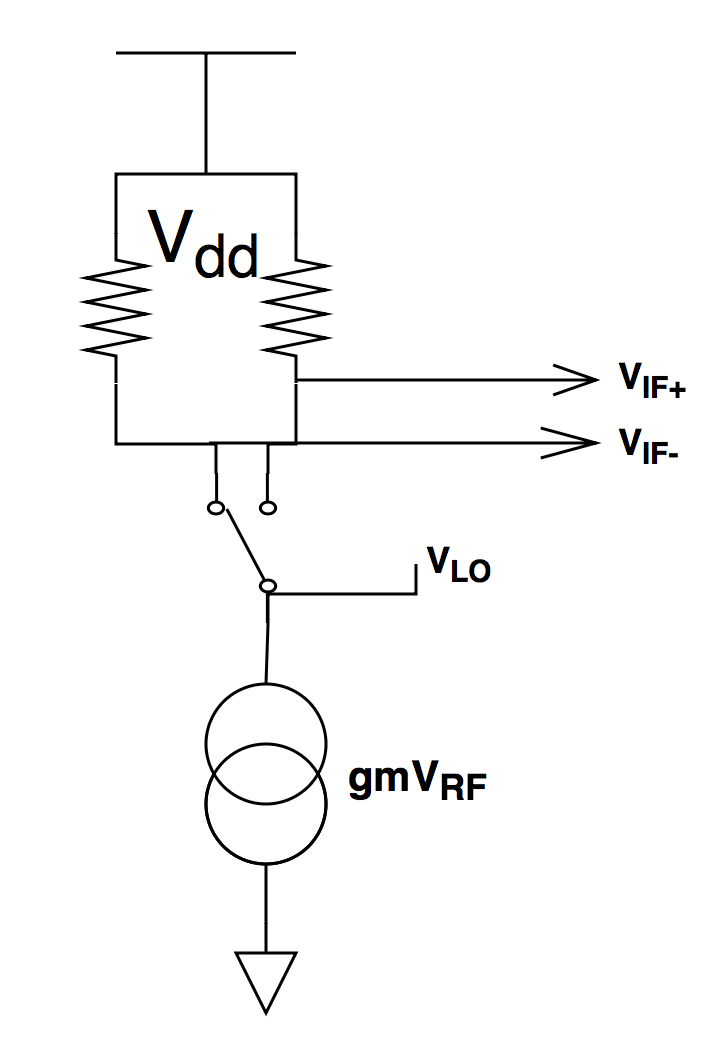
\includegraphics[width=0.3\textwidth] {Figures/gilbertSimple}
  \caption{Mixer Theory}
    \label{fig:simpmix}
\end{figure}

Since the Gilbert Cell is a double balanced i.e. both RF and LO inputs are differential, the feedthroughs get subtracted out at IF therefore
there should be very little of the RF and LO frequencies at the output.

\subsection{RF Port Matching}
Originally, as mentioned, the RF port was going to be matched with a 50 ohm source resistor. After understanding that the
matching of this circuit could be designed using the same methodology as a source-degenerated LNA topology and also encountering
voltage headroom problems, it became apparent that using source and gate inductors to match was the best option. The source inductor is used to match to 50 ohm
and the source and gate inductors combined are used to resonate out $C_{gs}$ (and in the case of high frequency many other parasitics).
\begin{equation}
  \label{eq:InputRes}
  50 \Omega = \omega_TLs
\end{equation}
\begin{equation}
  \label{eq:GateInd}
  \dfrac{1}{w(sC_{gs}+C_{others})} = \omega(L_s+L_g)
\end{equation}

For 65nm technology $\omega_T \approx 2\pi \times \omega_T$ REF. This is derived by assuming that impedance looking into the common gate (LO) stage is high,
it also ignores all other capacitances and $g_ds$ of RF transistors. \\

This method is greatly oversimplified for an 80GHz circuit, seeing as there are parasitic capacitances and finite output resistance. Therefore an attempt is made to create an improved input impedance model. Then initial values
are calculated using both models. After the simulated values are finalized there is a discussion outlining whether the improved model was useful.

\subsection{IF Port Matching}
 The output matching circuit was originally conceived to be resistive. Again, after I actually learned how to design this circuit,
 it became clear that an LC tank was required. Therefore the tank was designed to resonate at the desired frequency and the resistive
 load chosen to meet the output impedance requirement. As will be discussed in the simulation section, none of these values were as expected
 because of finite $g_{ds}$ and parasitics.

\subsection{Conversion Gain}

\newpage
\begin{landscape}

\section{Design Variations and Final Circuit Schematic}
\subsection{Circuit Schematic}

\begin{figure}[H]
  \centering
  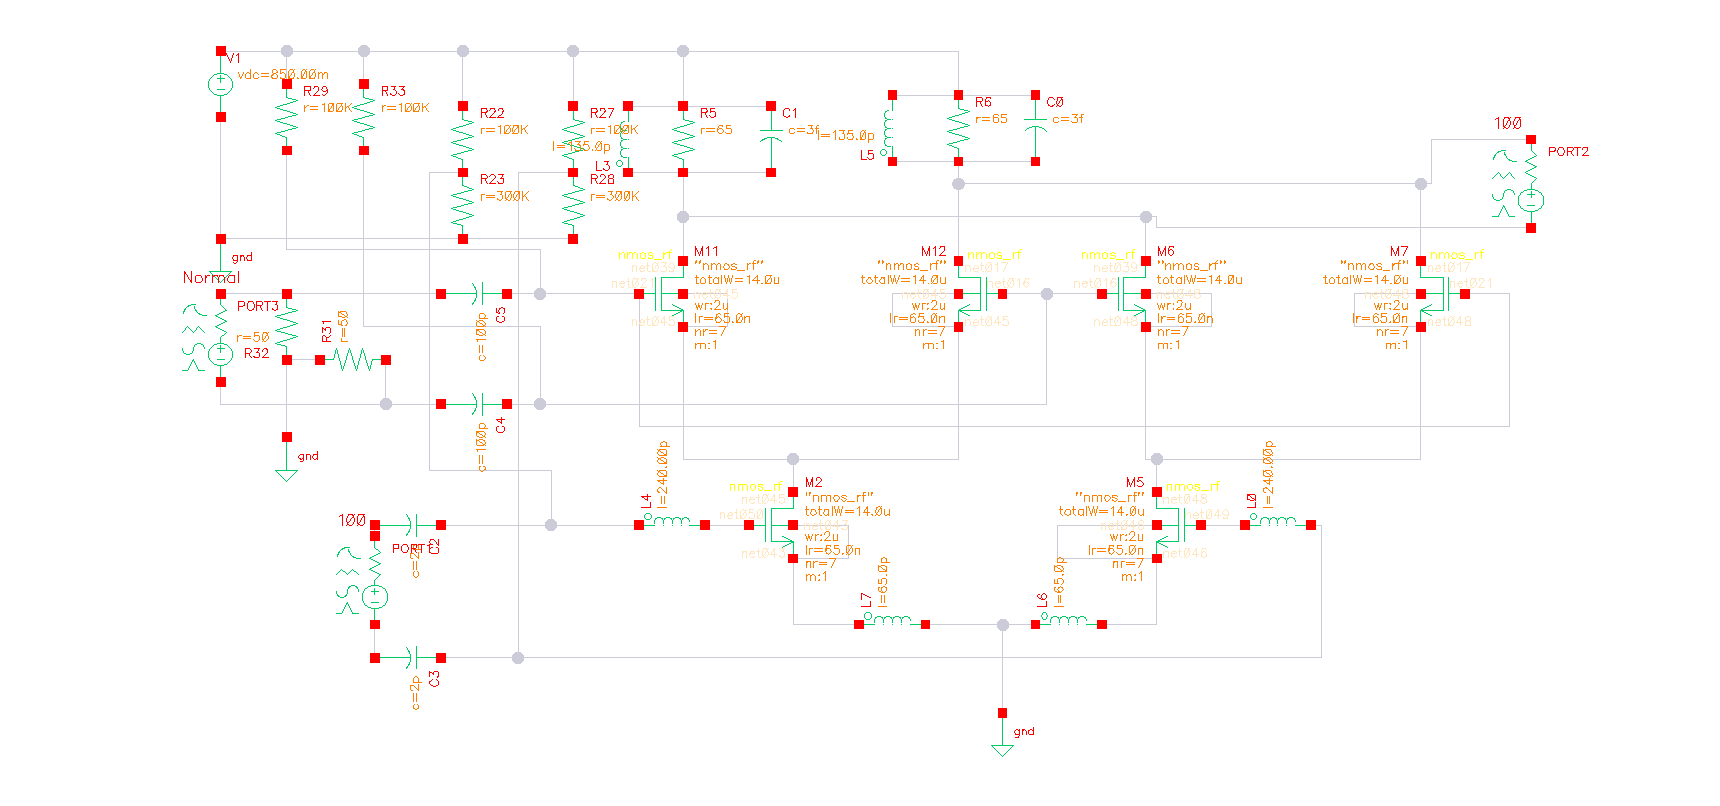
\includegraphics[width=1.5\textwidth] {Figures/Circuit.png}
  \caption{Final Design}
    \label{fig:finalschem}
\end{figure}
\end{landscape}
\newpage
At first the circuit was designed with a 1.8V power supply and a current mirror for biasing
as seen in figure X. However, this topology was causing many problems. First of all, node X
had to be maintained at $\approx$ 0.4V for the current mirror to function properly. This was
causing a lot of problems because of voltage headroom and being able to design for a $V_{od}$
of $\approx$ 0.1V while also staying under the power budget of 5mW. Therefore after (many weeks)
of using that topology, I realized I could scrap the current mirror and lower the voltage. An LC
tank was also added to increase voltage headroom and it later became apparent that those components would
also be required for output matching because of all the parasitics present.
This then allowed me to increase the widths of the transistor, therefore increases the transconductance
while still staying below the allotted power budget. The original transconductance was around 5mA/V while,
as mentioned, the overdrive voltage was around 50mV (not good). After the supply voltage/topology change
was implemented the transconductance achieved was WHAT NUMBA as shown in table BLAH
At first, an output resistance of 730$\Omega$
was chosen to give approximately 5dB of gain based on fig REF. However, it was decided that it would
be unusual to have such a high output impedance since in practice this device would need to interface
with other components (PA). Therefore the target was reduced to 50$\Omega$. The reduction in gain was
somewhat compensated by the fact that I was now able to get a bigger gm with the reduced power supply.


\section{Simulated Results}
\begin{table}[H]
  \small
  \centering
  \caption{Experiment Results-I}
  \subfloat[RF Transistors]{%
    \hspace{.5cm}%
    \begin{tabular}{|c|c|}
      \hline
      \textbf{Parameter} & \textbf{Value} \\
      \hline
      \hline
      $I_D$ &  2.819mA \\
      \hline
      $C_{gs}$ &  9.468fF \\
      \hline
      $C_{gd}$ &  3.613fF \\
      \hline
      $g_m$ &  14.94mA/V \\
      \hline
      $g_{ds}$ &  2.94mA/V \\
      \hline
      $V_{ds}$ &  331mV \\
      \hline
      $V_{gs}$ &  646mV \\
      \hline
      $V_{th}$ &  414mV \\
      \hline
      \hline
    \end{tabular}%
    \hspace{.5cm}%
  }\hspace{1cm}
  \subfloat[LO Transistors]{%
    \hspace{.5cm}%
    \begin{tabular}{|c|c|}
      \hline
      \textbf{Parameter} & \textbf{Value} \\
      \hline
      \hline
      $I_D$ &  1.409mA \\
      \hline
      $C_{gs}$ &  8.754fF \\
      \hline
      $C_{gd}$ &  3.216fF \\
      \hline
      $g_m$ &  12.18mA/V \\
      \hline
      $g_{ds}$ &  1.38mA/V \\
      \hline
      $V_{ds}$ &  510mV \\
      \hline
      $V_{gs}$ &  511mV \\
      \hline
      $V_{th}$ &  402mV \\
      \hline
      \hline
    \end{tabular}%
    \hspace{.5cm}%
  }
\end{table}

Overdrive voltage for LO transistors was lower than RF transistors. This is because it was important
that the LO transistors would fall into Triode and Cutoff when Max/Min LO was used and the overdrive
voltage for the RF transistors was designed high to get high transconductance while still remaining in saturation.
\subsection{Transistor Biasing and Power Consumption}

\subsection{Conversion Gain}
\begin{figure}[H]
  \centering
  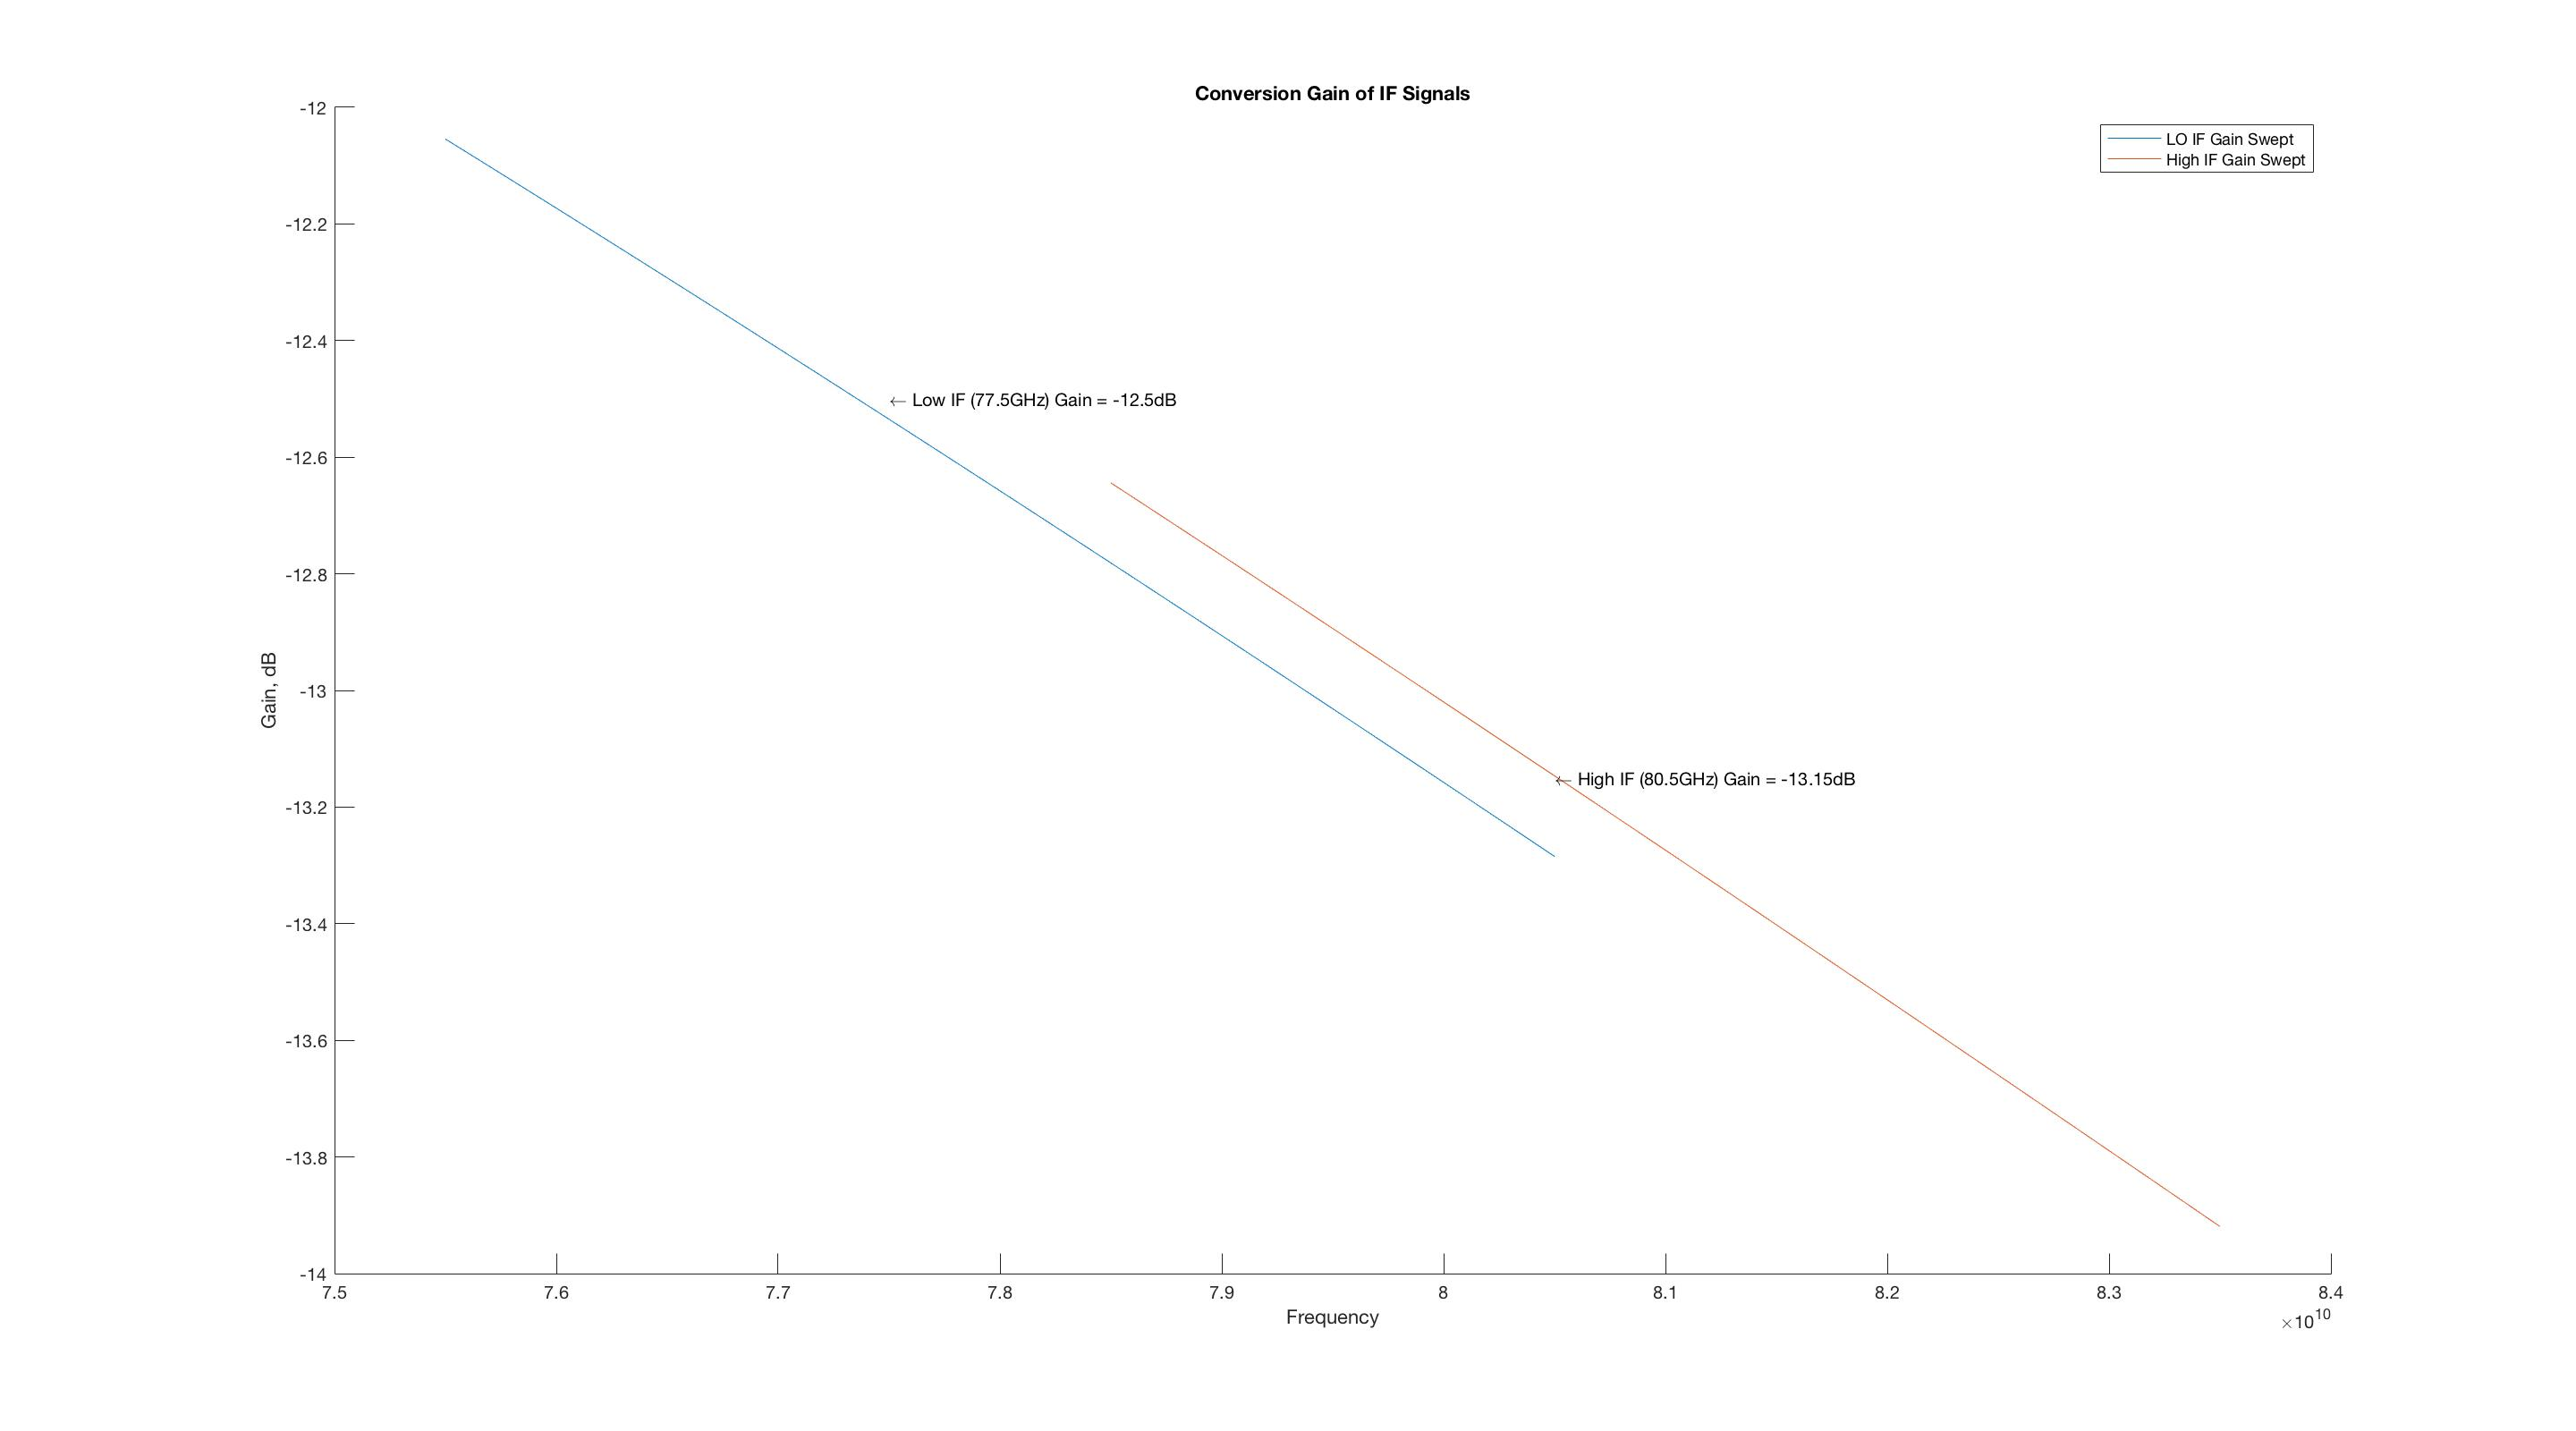
\includegraphics[width=0.95\textwidth] {Plots/Gain.jpg}
  \caption{Swept Gain for Lo and Hi IF}
    \label{fig:matgain}
\end{figure}
\subsection{Input and Output Matching}
\subsubsection{Theory}
As previously discussed, the source degenerated topology input impedance is defined by the
simple circuit seen below.

\begin{figure}[H]
  \centering
  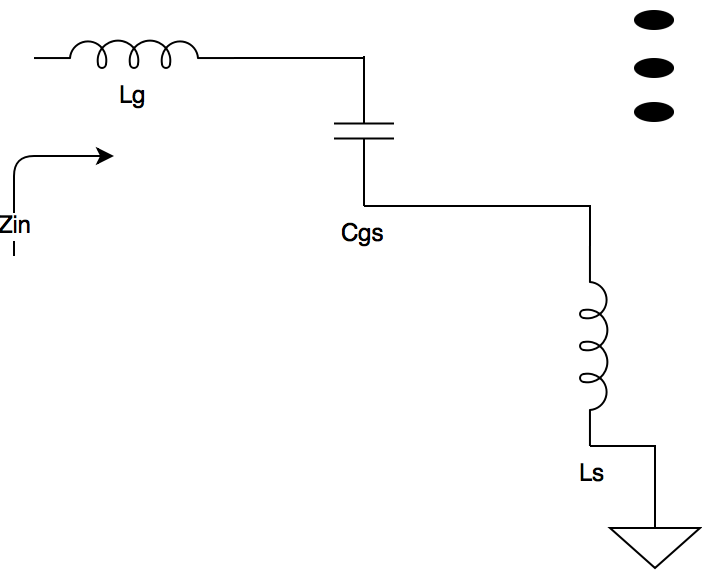
\includegraphics[width=0.3\textwidth] {Figures/zin}
  \caption{Simplified Input Impedance}
    \label{fig:zinSimple}
\end{figure}

From this model, Initial values of 50pH and 370pH are picked based on the simulated bias value of
$C_{gs}$.

Now, if we were to use the improved model of input impedance than we choose.

After itterative simulation the values OF VALUES were picked. Which model was more accurate!

\subsubsection{Results}
Excellent matching is achieved as shown in Figure ~\ref{fig:matS11}
\begin{figure}[H]
  \centering
  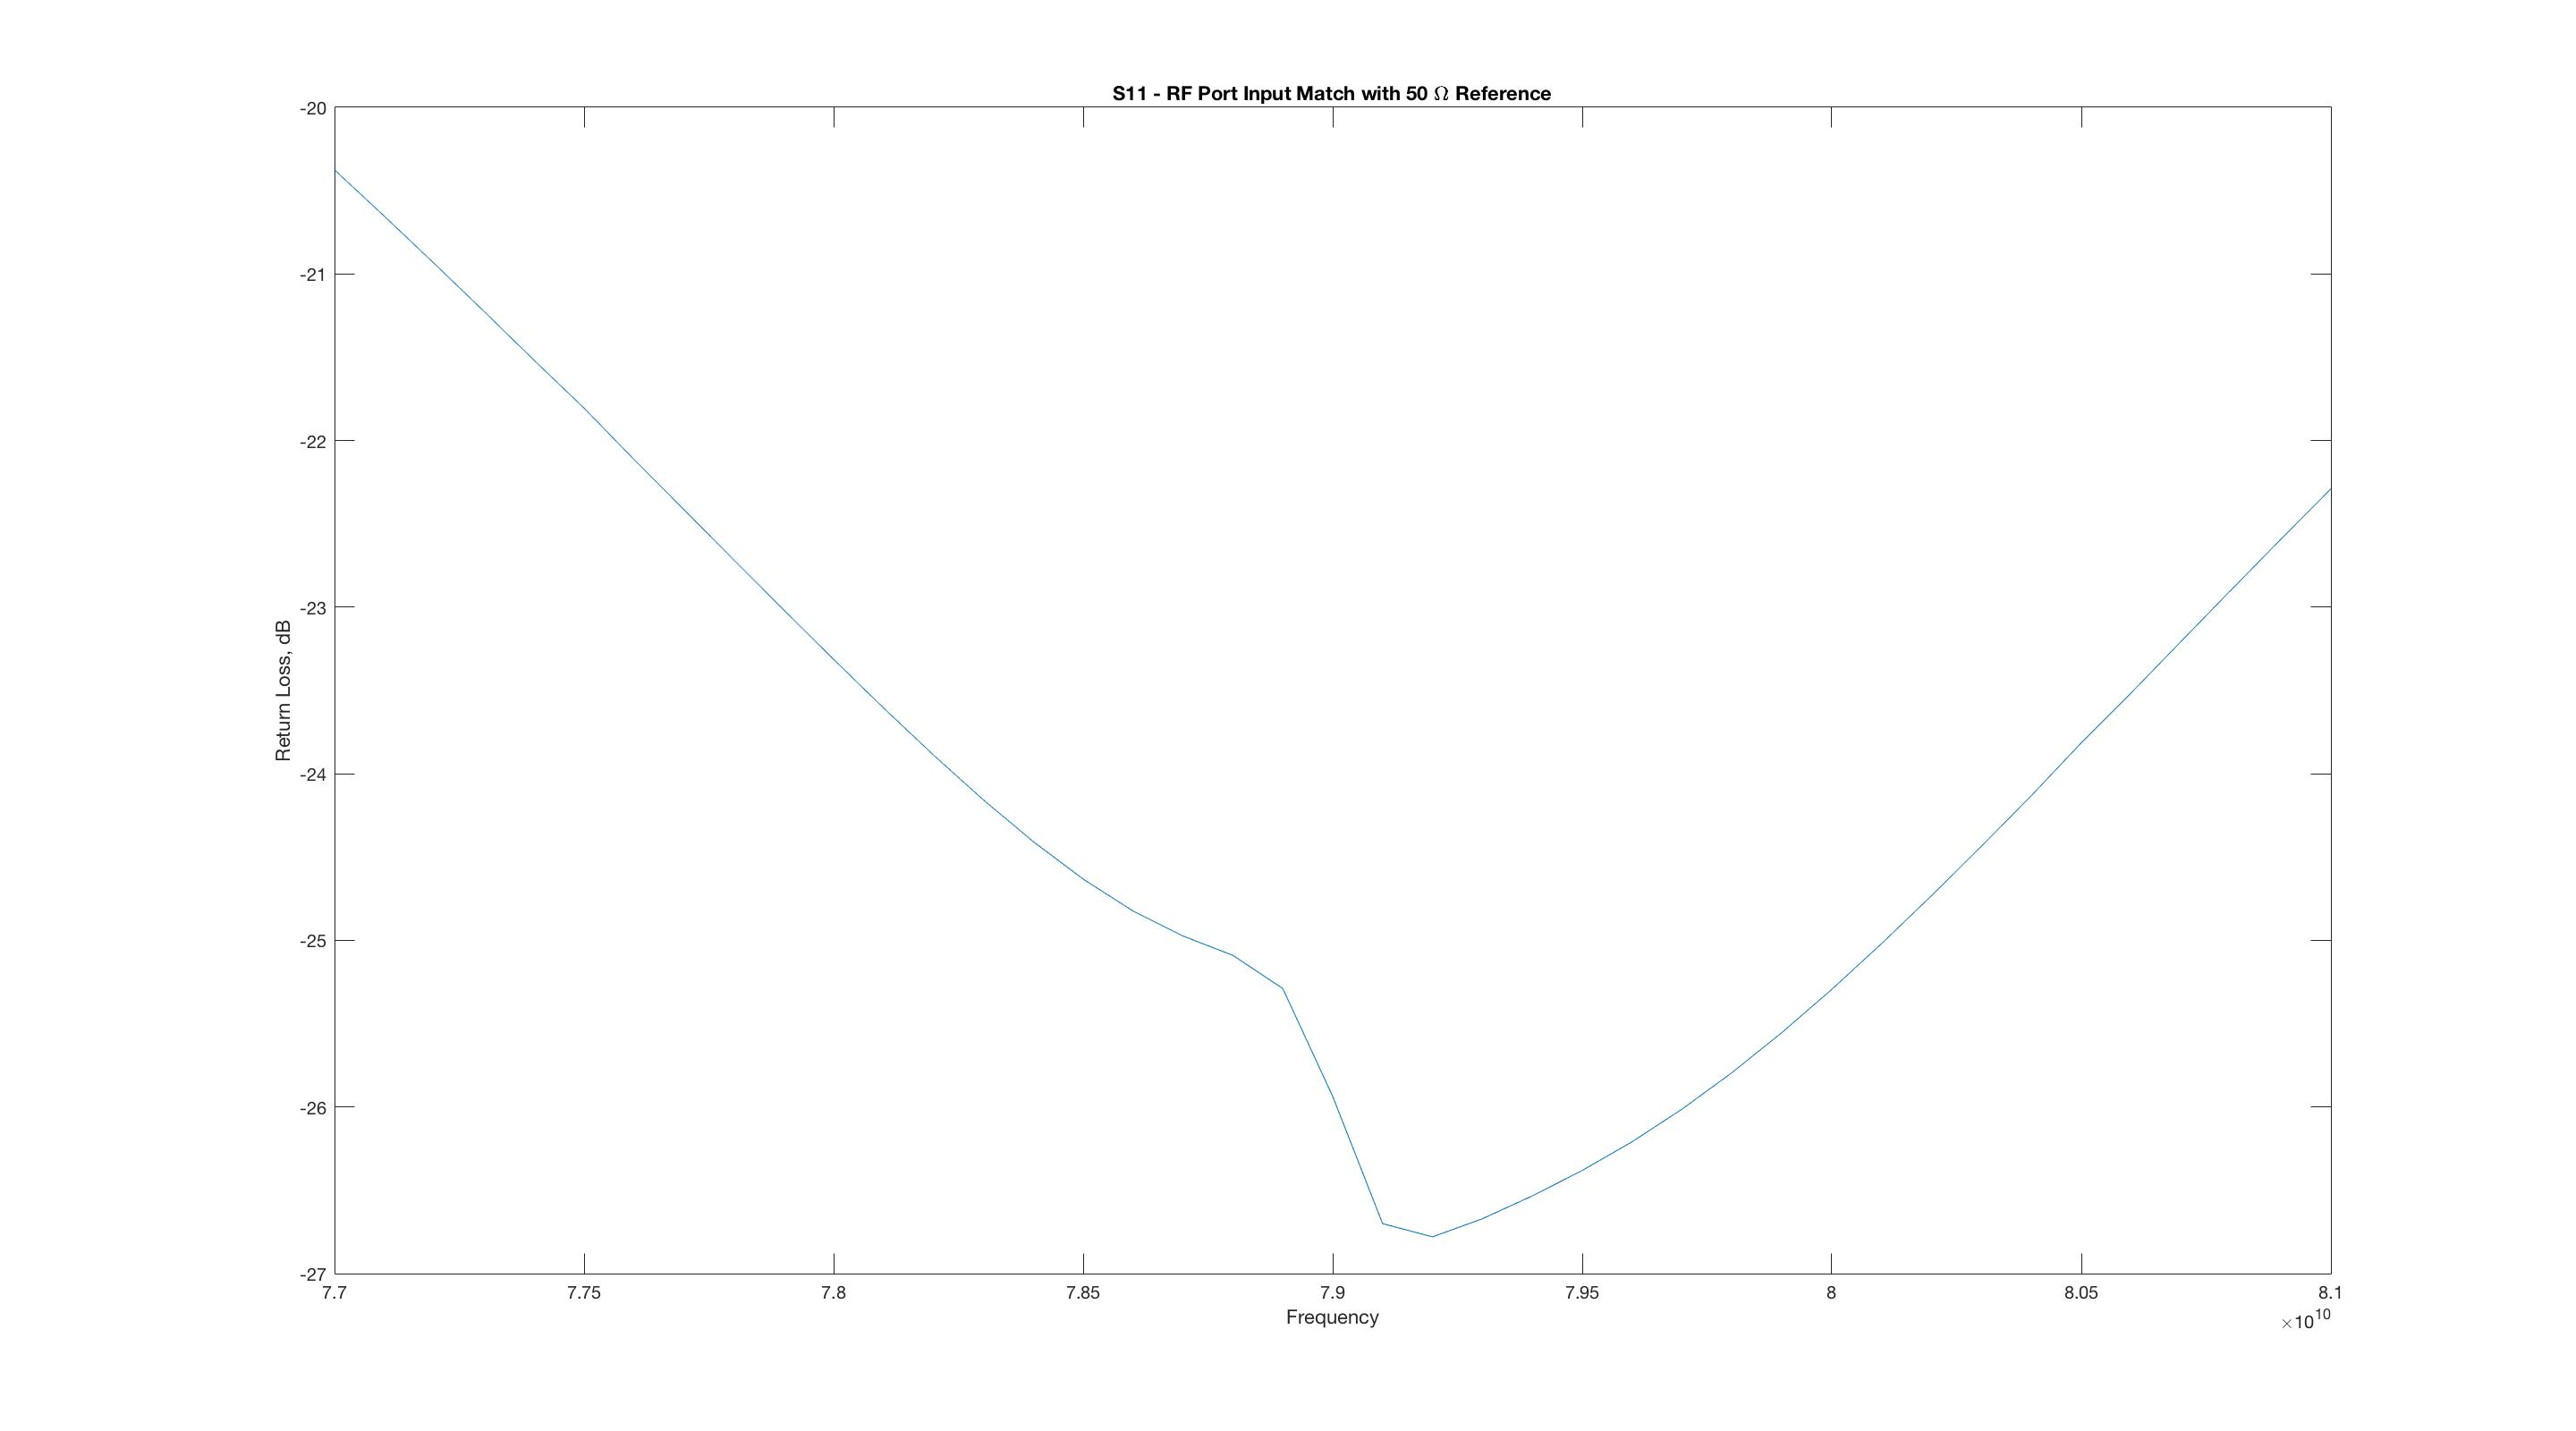
\includegraphics[width=0.95\textwidth] {Plots/S11.jpg}
  \caption{Final Return Loss of RF Port}
    \label{fig:matS11}
\end{figure}
\begin{figure}[H]
  \centering
  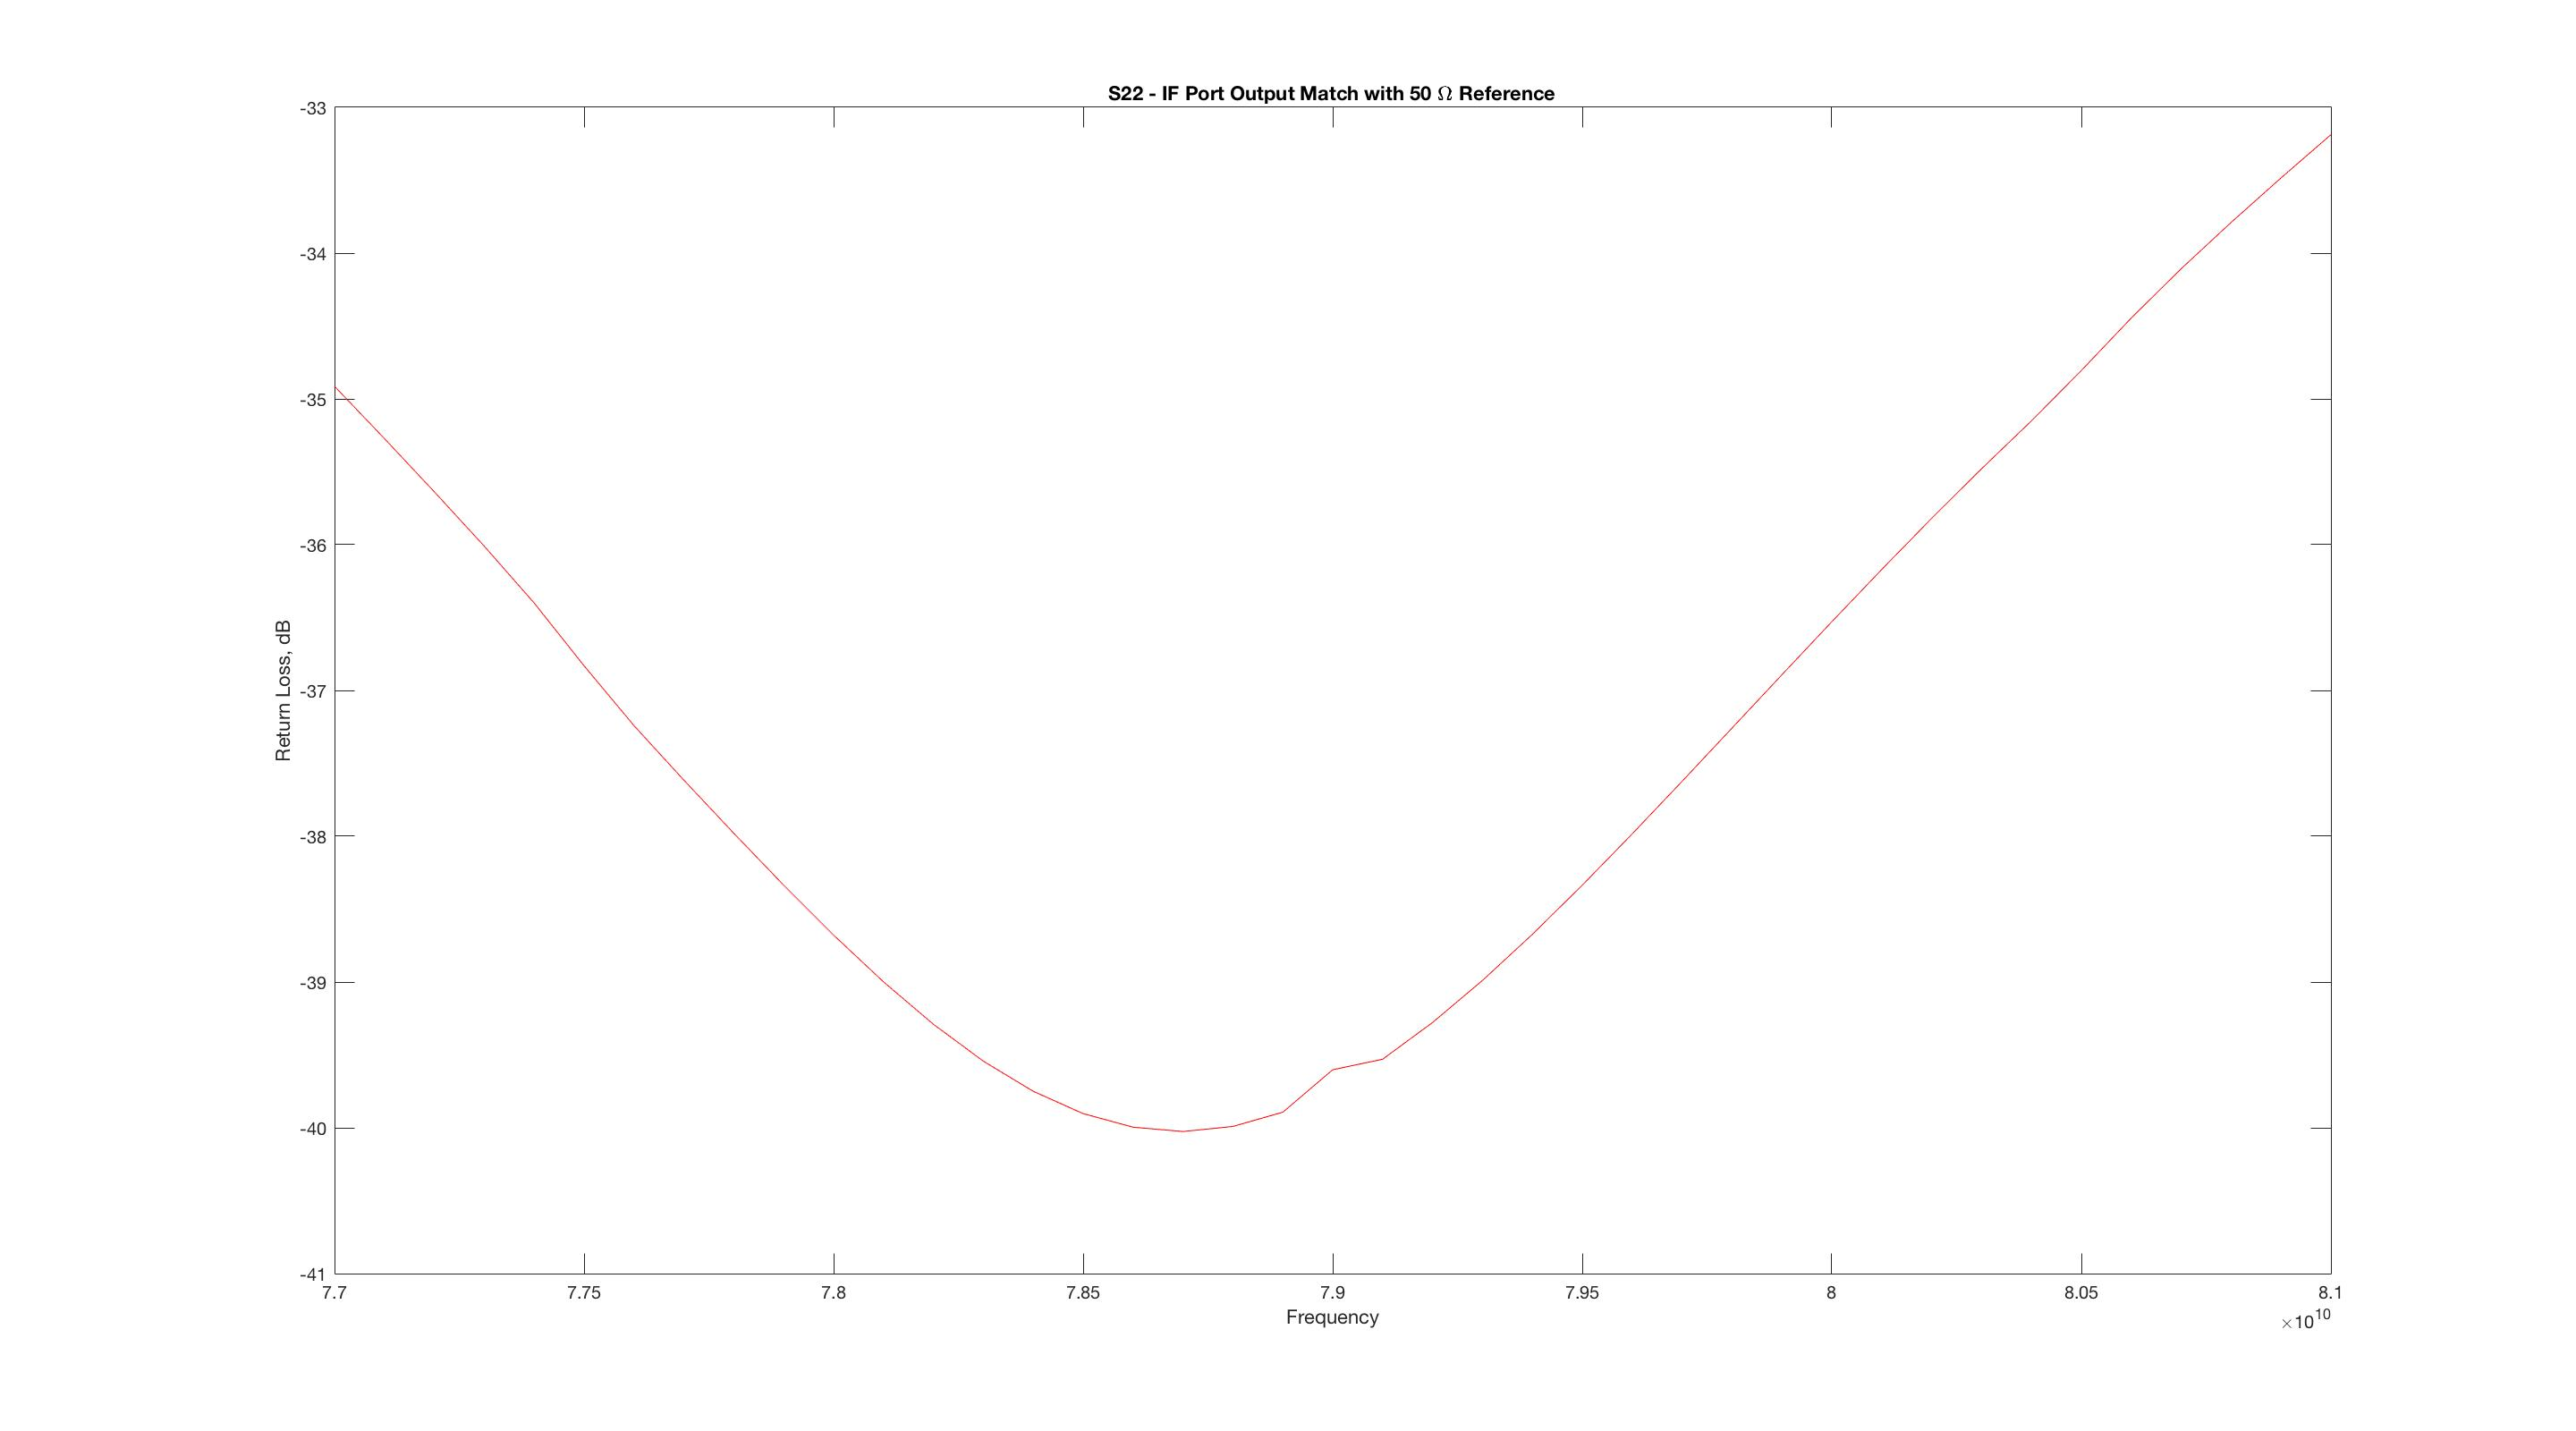
\includegraphics[width=0.95\textwidth] {Plots/S22.jpg}
  \caption{Final Return Loss of IF Port}
    \label{fig:matS22}
\end{figure}

The matching for the LO ports is simply done with 2 $50 \Omega$ resistors. Simulations
showed almost infinitely small return loss as expected.
\subsection{Noise Figure}
\begin{figure}[H]
  \centering
  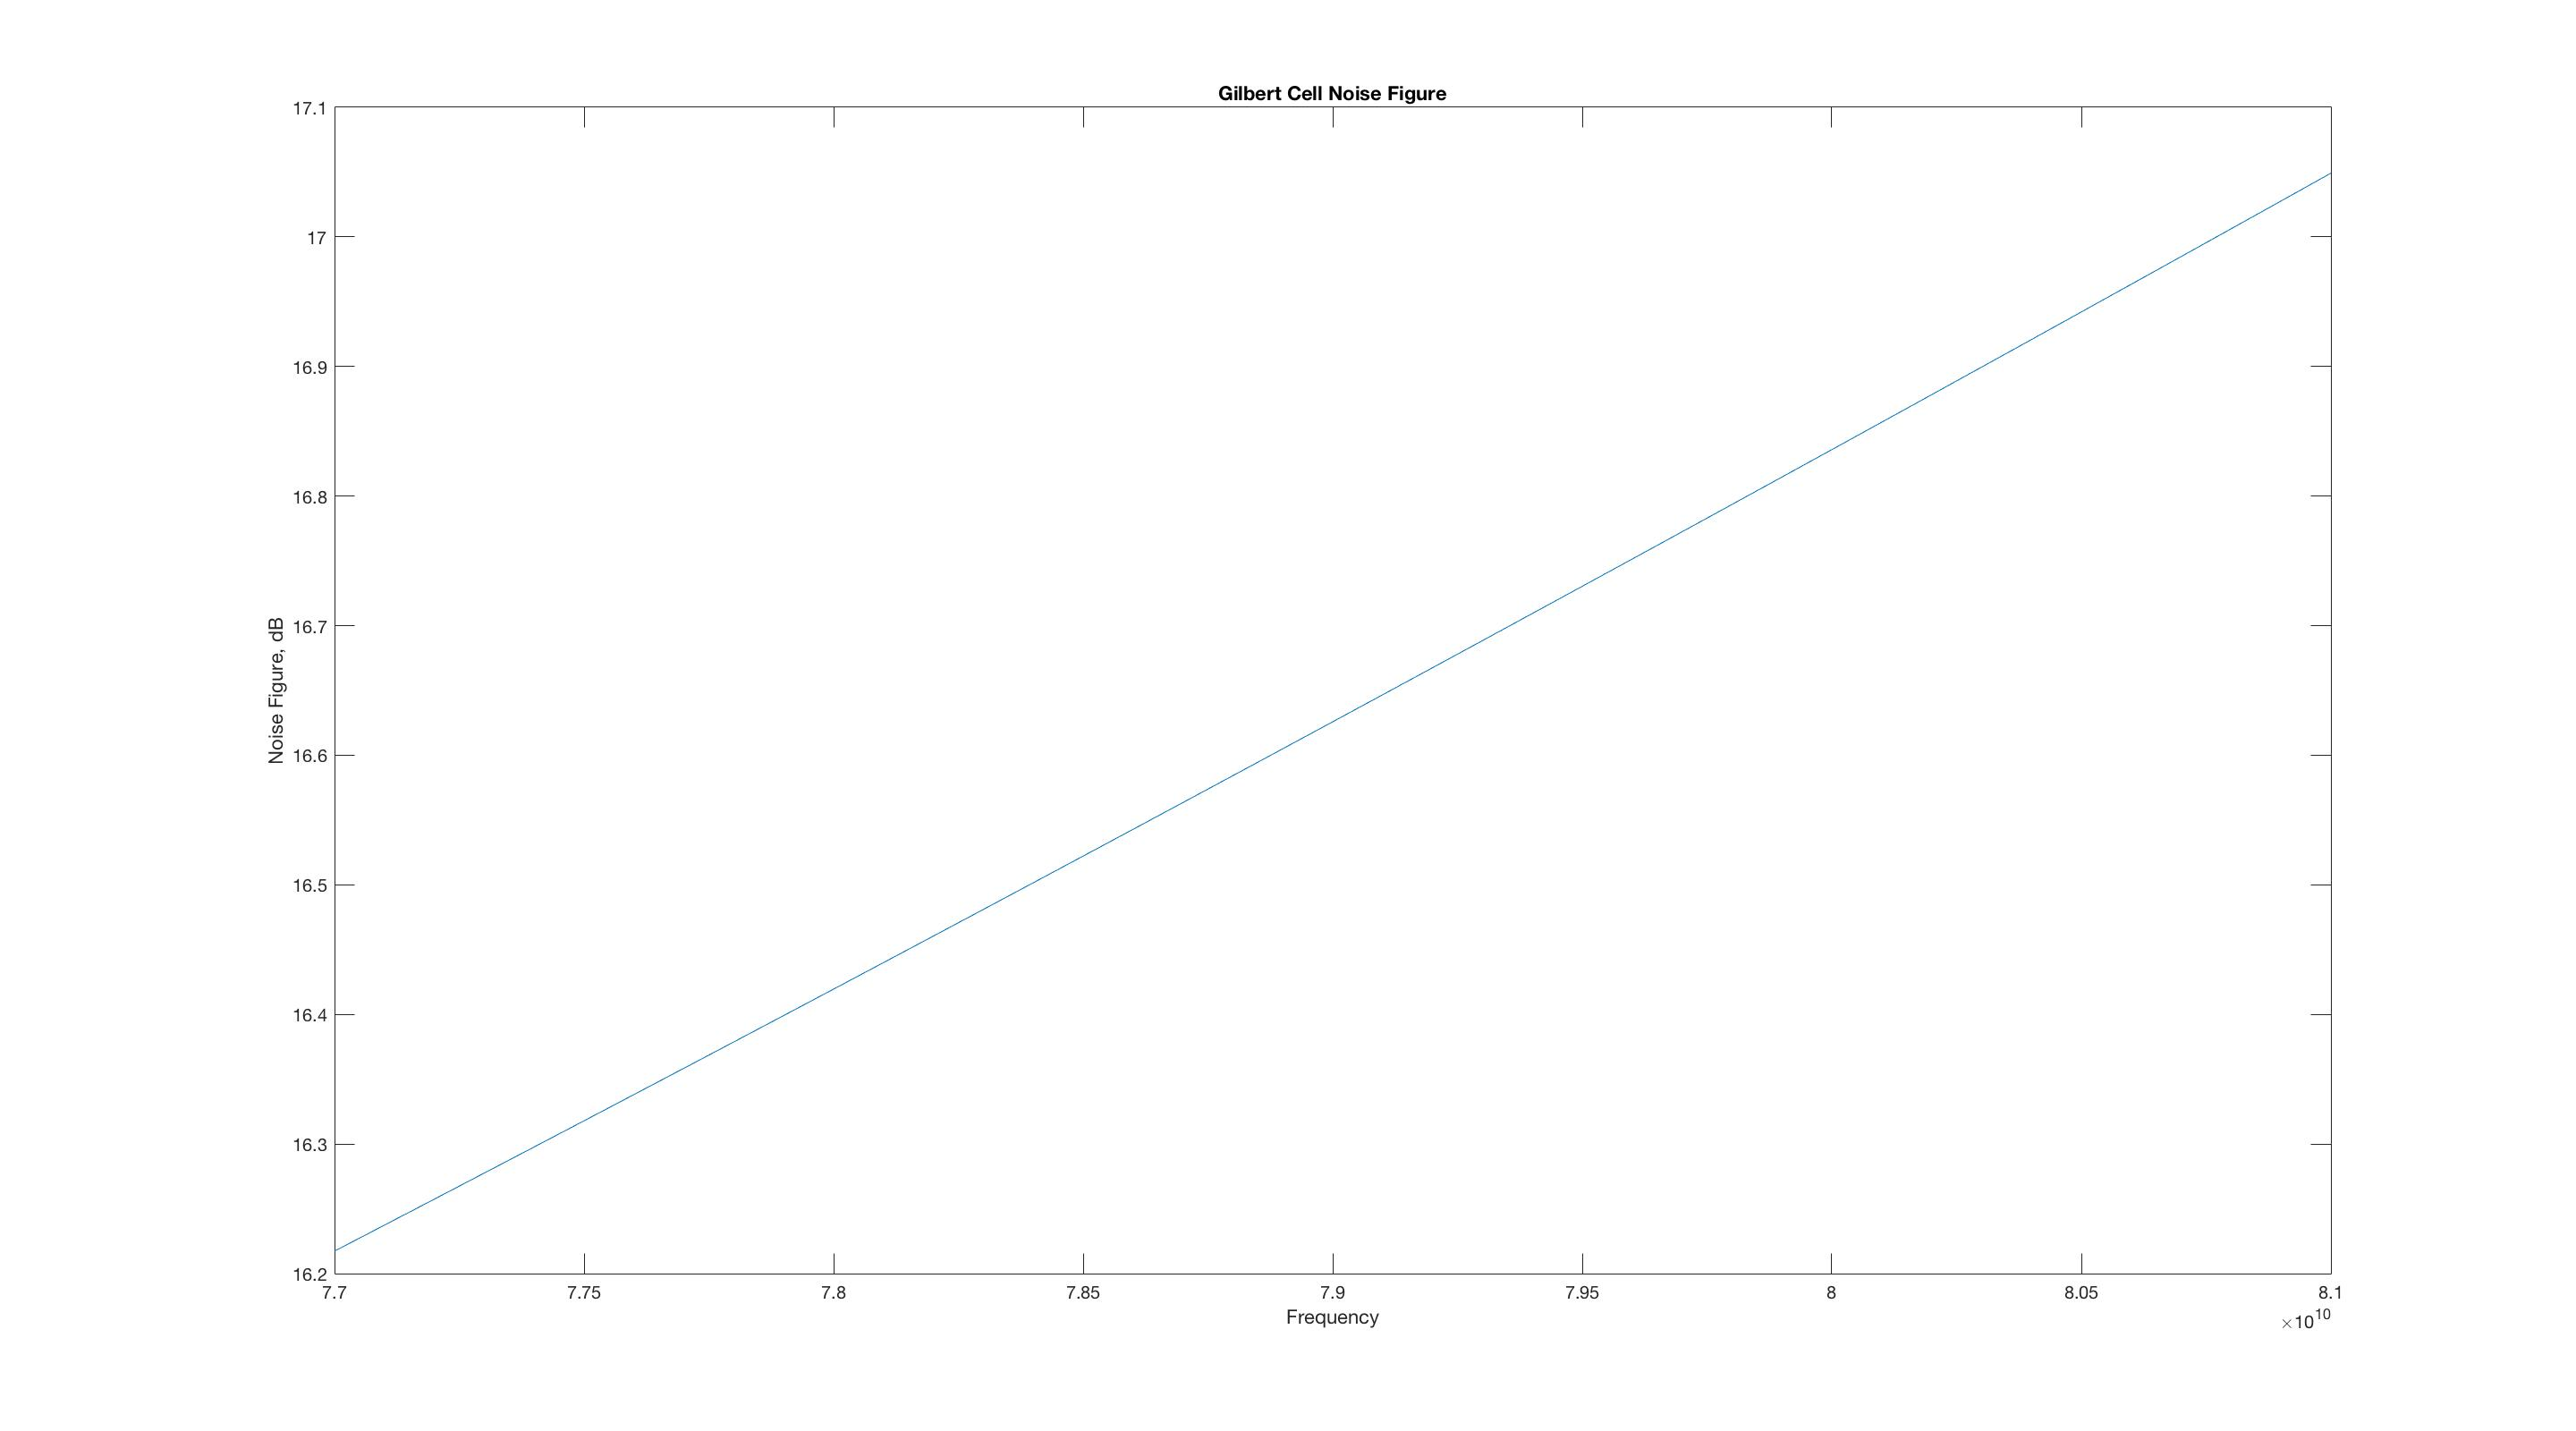
\includegraphics[width=0.95\textwidth] {Plots/NF.jpg}
  \caption{Final NF}
    \label{fig:matNF}
\end{figure}

\subsection{P1dB \& IP3}
Write some stuff about this...
\newpage
\section{Discussion}
\subsection{Future Improvements}


%----------------------------------------------------------------------------------------
%	REFERENCES
%----------------------------------------------------------------------------------------
\section{References}
\printbibliography[heading=none]

\newpage
%----------------------------------------------------------------------------------------
%	APPENDIX
%---------------------------------------------------------------------------------------
\begin{appendices}
\section{Cadence Simulation Plots}\label{app:cresults}
\subsection{Conversion Gain}
\begin{figure}[H]
  \centering
  \includegraphics[width=0.95\textwidth] {Figures/FinalConversionGain.bmp}
  \caption{Conversion Gain Cadence}
    \label{fig:cGain}
\end{figure}
\subsection{RMS Spectrum}
\begin{figure}[H]
  \centering
  \includegraphics[width=0.95\textwidth] {Figures/FinalSpectrum.bmp}
  \caption{RMS Spectrum Cadence}
    \label{fig:cSpectrum}
\end{figure}
\subsection{Noise Figure}
\begin{figure}[H]
  \centering
  \includegraphics[width=0.95\textwidth] {Figures/FinalNF.bmp}
  \caption{Noise Figure Cadence}
    \label{fig:cNF}
\end{figure}
\subsection{P1dB}
\begin{figure}[H]
  \centering
  \includegraphics[width=0.95\textwidth] {Figures/P1dB_GOOD_ATTEMPT1_77point5.bmp}
  \caption{P1dB Cadence}
    \label{fig:cP1db}
\end{figure}
\subsection{IP3}
\begin{figure}[H]
  \centering
  \includegraphics[width=0.95\textwidth] {Figures/IP3dB_GOOD_ATTEMPT1.bmp}
  \caption{IP3 Cadence}
    \label{fig:cIP3}
\end{figure}
\subsection{S11}
\begin{figure}[H]
  \centering
  \includegraphics[width=0.95\textwidth] {Figures/FinalS11_rect.bmp}
  \caption{RF Port Match}
    \label{fig:cS11}
\end{figure}
\subsection{S22}
\begin{figure}[H]
  \centering
  \includegraphics[width=0.95\textwidth] {Figures/FinalS22Rect.bmp}
  \caption{IF Port Match}
    \label{fig:cS22}
\end{figure}


\end{appendices}

\end{document}
